%%%% Paramétrage du TD %%%%
\def\xxactivite{ \ifprof \normalsize{TD 3 -- Corrigé } \else  \ifcolle Colle \else TD 3\fi \fi} % \normalsize \vspace{-.4cm}
\def\xxauteur{\textsl{Xavier Pessoles}}


\def\xxnumchapitre{Chapitre 1 \vspace{.2cm}}
\def\xxchapitre{\hspace{.12cm} Approche énergétique}

\def\xxcompetences{%
\vspace{-.5cm}
\footnotesize{
\textsl{%
\textbf{Savoirs et compétences :}\\
\vspace{-.2cm}
\begin{itemize}[label=\ding{112},font=\color{ocre}] 
\item Mod2.C18.SF1 : Déterminer l’énergie cinétique d’un solide, ou d’un ensemble de solides, dans son mouvement par rapport à un autre solide.
\item Res1.C1.SF1 : Proposer une démarche permettant la détermination de la loi de mouvement.
%\item Mod1.C5.SF2 : Déterminer la puissance des actions mécaniques extérieures à un solide ou à un ensemble de solides, dans son mouvement rapport à un autre solide.
%\item Mod1.C5.SF3 : Déterminer la puissance des actions mécaniques intérieures à un ensemble de solides.
\end{itemize}}}}


\def\xxtitreexo{Renault Twizy \ifnormal $\star$ \else \fi \iftdifficile $\star\star\star$ \else \fi }
\def\xxsourceexo{\hspace{.2cm} \footnotesize{Concours Commun Mines Ponts 2017}}

\def\xxfigures{
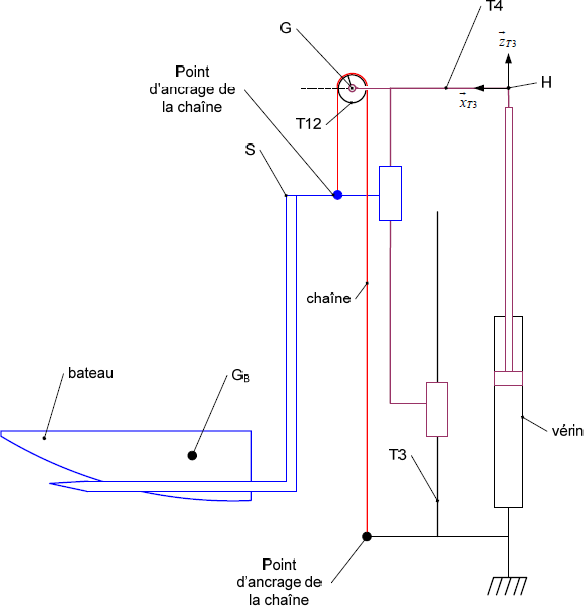
\includegraphics[width=.8\textwidth]{fig_01}
}%figues de la page de garde


\iflivret
\pagestyle{empty}


%%%%%%%% PAGE DE GARDE COURS
\ifcours
% ==== BANDEAU DES TITRES ==== 
\begin{tikzpicture}[remember picture,overlay]
\node at (current page.north west)
{\begin{tikzpicture}[remember picture,overlay]
\node[anchor=north west,inner sep=0pt] at (0,0) {\includegraphics[width=\paperwidth]{\thechapterimage}};
\draw[anchor=west] (-2cm,-8cm) node [line width=2pt,rounded corners=15pt,draw=ocre,fill=white,fill opacity=0.6,inner sep=40pt]{\strut\makebox[22cm]{}};
\draw[anchor=west] (1cm,-8cm) node {\huge\sffamily\bfseries\color{black} %
\begin{minipage}{1cm}
\rotatebox{90}{\LARGE\sffamily\textsc{\color{ocre}\textbf{\xxnumpartie}}}
\end{minipage} \hfill
\begin{minipage}[c]{14cm}
\begin{titrepartie}
\begin{flushright}
\renewcommand{\baselinestretch}{1.1} 
\Large\sffamily\textsc{\textbf{\xxpartie}}
\renewcommand{\baselinestretch}{1} 
\end{flushright}
\end{titrepartie}
\end{minipage} \hfill
\begin{minipage}[c]{3.5cm}
{\large\sffamily\textsc{\textbf{\color{ocre} \discipline}}}
\end{minipage} 
 };
\end{tikzpicture}};
\end{tikzpicture}
% ==== FIN BANDEAU DES TITRES ==== 


% ==== ONGLET 
\begin{tikzpicture}[overlay]
\node[shape=rectangle, 
      rounded corners = .25 cm,
	  draw= ocre,
	  line width=2pt, 
	  fill = ocre!10,
	  minimum width  = 2.5cm,
	  minimum height = 3cm,] at (18.3cm,0) {};
\node at (17.7cm,0) {\rotatebox{90}{\textbf{\Large\color{ocre}{\classe}}}};
%{};
\end{tikzpicture}
% ==== FIN ONGLET 


\vspace{3.5cm}

\begin{tikzpicture}[remember picture,overlay]
\draw[anchor=west] (-2cm,-6cm) node {\huge\sffamily\bfseries\color{black} %
\begin{minipage}{2cm}
\begin{center}
\LARGE\sffamily\textsc{\color{ocre}\textbf{\xxactivite}}
\end{center}
\end{minipage} \hfill
\begin{minipage}[c]{15cm}
\begin{titrechapitre}
\renewcommand{\baselinestretch}{1.1} 
\Large\sffamily\textsc{\textbf{\xxnumchapitre}}

\Large\sffamily\textsc{\textbf{\xxchapitre}}
\vspace{.5cm}

\renewcommand{\baselinestretch}{1} 
\normalsize\normalfont
\xxcompetences
\end{titrechapitre}
\end{minipage}  };
\end{tikzpicture}
\vfill

\begin{flushright}
\begin{minipage}[c]{.3\linewidth}
\begin{center}
\xxfigures
\end{center}
\end{minipage}\hfill
\begin{minipage}[c]{.6\linewidth}
\startcontents
%\printcontents{}{1}{}
\printcontents{}{1}{}
\end{minipage}
\end{flushright}

\begin{tikzpicture}[remember picture,overlay]
\draw[anchor=west] (4.5cm,-.7cm) node {
\begin{minipage}[c]{.2\linewidth}
\begin{flushright}

\includegraphics[width=2cm]{logoCC}
\end{flushright}
\end{minipage}
\begin{minipage}[c]{.2\linewidth}
\textsl{\xxauteur} \\
\textsl{\classe}
\end{minipage}
 };
\end{tikzpicture}

\newpage
\pagestyle{fancy}

%\newpage
%\pagestyle{fancy}

\else
\fi
%% FIN PAGE DE GARDE DES COURS

%%%%%%%% PAGE DE GARDE TD
\iftd
%\begin{tikzpicture}[remember picture,overlay]
%\node at (current page.north west)
%{\begin{tikzpicture}[remember picture,overlay]
%\draw[anchor=west] (-2cm,-3.25cm) node [line width=2pt,rounded corners=15pt,draw=ocre,fill=white,fill opacity=0.6,inner sep=40pt]{\strut\makebox[22cm]{}};
%\draw[anchor=west] (1cm,-3.25cm) node {\huge\sffamily\bfseries\color{black} %
%\begin{minipage}{1cm}
%\rotatebox{90}{\LARGE\sffamily\textsc{\color{ocre}\textbf{\xxnumpartie}}}
%\end{minipage} \hfill
%\begin{minipage}[c]{13.5cm}
%\begin{titrepartie}
%\begin{flushright}
%\renewcommand{\baselinestretch}{1.1} 
%\Large\sffamily\textsc{\textbf{\xxpartie}}
%\renewcommand{\baselinestretch}{1} 
%\end{flushright}
%\end{titrepartie}
%\end{minipage} \hfill
%\begin{minipage}[c]{3.5cm}
%{\large\sffamily\textsc{\textbf{\color{ocre} \discipline}}}
%\end{minipage} 
% };
%\end{tikzpicture}};
%\end{tikzpicture}

%%%%%%%%%% PAGE DE GARDE TD %%%%%%%%%%%%%%%
%\begin{tikzpicture}[overlay]
%\node[shape=rectangle, 
%      rounded corners = .25 cm,
%	  draw= ocre,
%	  line width=2pt, 
%	  fill = ocre!10,
%	  minimum width  = 2.5cm,
%	  minimum height = 2.5cm,] at (18.5cm,0) {};
%\node at (17.7cm,0) {\rotatebox{90}{\textbf{\Large\color{ocre}{\classe}}}};
%%{};
%\end{tikzpicture}

% PARTIE ET CHAPITRE
%\begin{tikzpicture}[remember picture,overlay]
%\draw[anchor=west] (-1cm,-2.1cm) node {\large\sffamily\bfseries\color{black} %
%\begin{minipage}[c]{15cm}
%\begin{flushleft}
%\xxnumchapitre \\
%\xxchapitre
%\end{flushleft}
%\end{minipage}  };
%\end{tikzpicture}

% BANDEAU EXO
\iflivret % SI LIVRET
\begin{tikzpicture}[remember picture,overlay]
\draw[anchor=west] (-2cm,-3.3cm) node {\huge\sffamily\bfseries\color{black} %
\begin{minipage}{5cm}
\begin{center}
\LARGE\sffamily\color{ocre}\textbf{\textsc{\xxactivite}}

\begin{center}
\xxfigures
\end{center}

\end{center}
\end{minipage} \hfill
\begin{minipage}[c]{12cm}
\begin{titrechapitre}
\renewcommand{\baselinestretch}{1.1} 
\large\sffamily\textbf{\textsc{\xxtitreexo}}

\small\sffamily{\textbf{\textit{\color{black!70}\xxsourceexo}}}
\vspace{.5cm}

\renewcommand{\baselinestretch}{1} 
\normalsize\normalfont
\xxcompetences
\end{titrechapitre}
\end{minipage}};
\end{tikzpicture}
\else % ELSE NOT LIVRET
\begin{tikzpicture}[remember picture,overlay]
\draw[anchor=west] (-2cm,-4.5cm) node {\huge\sffamily\bfseries\color{black} %
\begin{minipage}{5cm}
\begin{center}
\LARGE\sffamily\color{ocre}\textbf{\textsc{\xxactivite}}

\begin{center}
\xxfigures
\end{center}

\end{center}
\end{minipage} \hfill
\begin{minipage}[c]{12cm}
\begin{titrechapitre}
\renewcommand{\baselinestretch}{1.1} 
\large\sffamily\textbf{\textsc{\xxtitreexo}}

\small\sffamily{\textbf{\textit{\color{black!70}\xxsourceexo}}}
\vspace{.5cm}

\renewcommand{\baselinestretch}{1} 
\normalsize\normalfont
\xxcompetences
\end{titrechapitre}
\end{minipage}};
\end{tikzpicture}

\fi

\else   % FIN IF TD
\fi


%%%%%%%% PAGE DE GARDE FICHE
\iffiche
\begin{tikzpicture}[remember picture,overlay]
\node at (current page.north west)
{\begin{tikzpicture}[remember picture,overlay]
\draw[anchor=west] (-2cm,-2.25cm) node [line width=2pt,rounded corners=15pt,draw=ocre,fill=white,fill opacity=0.6,inner sep=40pt]{\strut\makebox[22cm]{}};
\draw[anchor=west] (1cm,-2.25cm) node {\huge\sffamily\bfseries\color{black} %
\begin{minipage}{1cm}
\rotatebox{90}{\LARGE\sffamily\textsc{\color{ocre}\textbf{\xxnumpartie}}}
\end{minipage} \hfill
\begin{minipage}[c]{14cm}
\begin{titrepartie}
\begin{flushright}
\renewcommand{\baselinestretch}{1.1} 
\large\sffamily\textsc{\textbf{\xxpartie} \\} 

\vspace{.2cm}

\normalsize\sffamily\textsc{\textbf{\xxnumchapitre -- \xxchapitre}}
\renewcommand{\baselinestretch}{1} 
\end{flushright}
\end{titrepartie}
\end{minipage} \hfill
\begin{minipage}[c]{3.5cm}
{\large\sffamily\textsc{\textbf{\color{ocre} \discipline}}}
\end{minipage} 
 };
\end{tikzpicture}};
\end{tikzpicture}

\iflivret
\begin{tikzpicture}[overlay]
\node[shape=rectangle, 
      rounded corners = .25 cm,
	  draw= ocre,
	  line width=2pt, 
	  fill = ocre!10,
	  minimum width  = 2.5cm,
	  minimum height = 2.5cm,] at (18.5cm,1.1cm) {};
\node at (17.9cm,1.1cm) {\rotatebox{90}{\textsf{\textbf{\large\color{ocre}{\classe}}}}};
%{};
\end{tikzpicture}
\else
\begin{tikzpicture}[overlay]
\node[shape=rectangle, 
      rounded corners = .25 cm,
	  draw= ocre,
	  line width=2pt, 
	  fill = ocre!10,
	  minimum width  = 2.5cm,
%	  minimum height = 2.5cm,] at (18.5cm,1.1cm) {};
	  minimum height = 2.5cm,] at (18.6cm,0cm) {};
\node at (18cm,0cm) {\rotatebox{90}{\textsf{\textbf{\large\color{ocre}{\classe}}}}};
%{};
\end{tikzpicture}

\fi

\else
\fi



\else
\pagestyle{empty}


%%%%%%%% PAGE DE GARDE COURS
\ifcours
% ==== BANDEAU DES TITRES ==== 
\begin{tikzpicture}[remember picture,overlay]
\node at (current page.north west)
{\begin{tikzpicture}[remember picture,overlay]
\node[anchor=north west,inner sep=0pt] at (0,0) {\includegraphics[width=\paperwidth]{\thechapterimage}};
\draw[anchor=west] (-2cm,-8cm) node [line width=2pt,rounded corners=15pt,draw=ocre,fill=white,fill opacity=0.6,inner sep=40pt]{\strut\makebox[22cm]{}};
\draw[anchor=west] (1cm,-8cm) node {\huge\sffamily\bfseries\color{black} %
\begin{minipage}{1cm}
\rotatebox{90}{\LARGE\sffamily\textsc{\color{ocre}\textbf{\xxnumpartie}}}
\end{minipage} \hfill
\begin{minipage}[c]{14cm}
\begin{titrepartie}
\begin{flushright}
\renewcommand{\baselinestretch}{1.1} 
\Large\sffamily\textsc{\textbf{\xxpartie}}
\renewcommand{\baselinestretch}{1} 
\end{flushright}
\end{titrepartie}
\end{minipage} \hfill
\begin{minipage}[c]{3.5cm}
{\large\sffamily\textsc{\textbf{\color{ocre} \discipline}}}
\end{minipage} 
 };
\end{tikzpicture}};
\end{tikzpicture}
% ==== FIN BANDEAU DES TITRES ==== 


% ==== ONGLET 
\begin{tikzpicture}[overlay]
\node[shape=rectangle, 
      rounded corners = .25 cm,
	  draw= ocre,
	  line width=2pt, 
	  fill = ocre!10,
	  minimum width  = 2.5cm,
	  minimum height = 3cm,] at (18.3cm,0) {};
\node at (17.7cm,0) {\rotatebox{90}{\textbf{\Large\color{ocre}{\classe}}}};
%{};
\end{tikzpicture}
% ==== FIN ONGLET 


\vspace{3.5cm}

\begin{tikzpicture}[remember picture,overlay]
\draw[anchor=west] (-2cm,-6cm) node {\huge\sffamily\bfseries\color{black} %
\begin{minipage}{2cm}
\begin{center}
\LARGE\sffamily\textsc{\color{ocre}\textbf{\xxactivite}}
\end{center}
\end{minipage} \hfill
\begin{minipage}[c]{15cm}
\begin{titrechapitre}
\renewcommand{\baselinestretch}{1.1} 
\Large\sffamily\textsc{\textbf{\xxnumchapitre}}

\Large\sffamily\textsc{\textbf{\xxchapitre}}
\vspace{.5cm}

\renewcommand{\baselinestretch}{1} 
\normalsize\normalfont
\xxcompetences
\end{titrechapitre}
\end{minipage}  };
\end{tikzpicture}
\vfill

\begin{flushright}
\begin{minipage}[c]{.3\linewidth}
\begin{center}
\xxfigures
\end{center}
\end{minipage}\hfill
\begin{minipage}[c]{.6\linewidth}
\startcontents
%\printcontents{}{1}{}
\printcontents{}{1}{}
\end{minipage}
\end{flushright}

\begin{tikzpicture}[remember picture,overlay]
\draw[anchor=west] (4.5cm,-.7cm) node {
\begin{minipage}[c]{.2\linewidth}
\begin{flushright}

\includegraphics[width=2cm]{logoCC}
\end{flushright}
\end{minipage}
\begin{minipage}[c]{.2\linewidth}
\textsl{\xxauteur} \\
\textsl{\classe}
\end{minipage}
 };
\end{tikzpicture}

\newpage
\pagestyle{fancy}

%\newpage
%\pagestyle{fancy}

\else
\fi
%% FIN PAGE DE GARDE DES COURS

%%%%%%%% PAGE DE GARDE TD
\iftd
%\begin{tikzpicture}[remember picture,overlay]
%\node at (current page.north west)
%{\begin{tikzpicture}[remember picture,overlay]
%\draw[anchor=west] (-2cm,-3.25cm) node [line width=2pt,rounded corners=15pt,draw=ocre,fill=white,fill opacity=0.6,inner sep=40pt]{\strut\makebox[22cm]{}};
%\draw[anchor=west] (1cm,-3.25cm) node {\huge\sffamily\bfseries\color{black} %
%\begin{minipage}{1cm}
%\rotatebox{90}{\LARGE\sffamily\textsc{\color{ocre}\textbf{\xxnumpartie}}}
%\end{minipage} \hfill
%\begin{minipage}[c]{13.5cm}
%\begin{titrepartie}
%\begin{flushright}
%\renewcommand{\baselinestretch}{1.1} 
%\Large\sffamily\textsc{\textbf{\xxpartie}}
%\renewcommand{\baselinestretch}{1} 
%\end{flushright}
%\end{titrepartie}
%\end{minipage} \hfill
%\begin{minipage}[c]{3.5cm}
%{\large\sffamily\textsc{\textbf{\color{ocre} \discipline}}}
%\end{minipage} 
% };
%\end{tikzpicture}};
%\end{tikzpicture}

%%%%%%%%%% PAGE DE GARDE TD %%%%%%%%%%%%%%%
%\begin{tikzpicture}[overlay]
%\node[shape=rectangle, 
%      rounded corners = .25 cm,
%	  draw= ocre,
%	  line width=2pt, 
%	  fill = ocre!10,
%	  minimum width  = 2.5cm,
%	  minimum height = 2.5cm,] at (18.5cm,0) {};
%\node at (17.7cm,0) {\rotatebox{90}{\textbf{\Large\color{ocre}{\classe}}}};
%%{};
%\end{tikzpicture}

% PARTIE ET CHAPITRE
%\begin{tikzpicture}[remember picture,overlay]
%\draw[anchor=west] (-1cm,-2.1cm) node {\large\sffamily\bfseries\color{black} %
%\begin{minipage}[c]{15cm}
%\begin{flushleft}
%\xxnumchapitre \\
%\xxchapitre
%\end{flushleft}
%\end{minipage}  };
%\end{tikzpicture}

% BANDEAU EXO
\iflivret % SI LIVRET
\begin{tikzpicture}[remember picture,overlay]
\draw[anchor=west] (-2cm,-3.3cm) node {\huge\sffamily\bfseries\color{black} %
\begin{minipage}{5cm}
\begin{center}
\LARGE\sffamily\color{ocre}\textbf{\textsc{\xxactivite}}

\begin{center}
\xxfigures
\end{center}

\end{center}
\end{minipage} \hfill
\begin{minipage}[c]{12cm}
\begin{titrechapitre}
\renewcommand{\baselinestretch}{1.1} 
\large\sffamily\textbf{\textsc{\xxtitreexo}}

\small\sffamily{\textbf{\textit{\color{black!70}\xxsourceexo}}}
\vspace{.5cm}

\renewcommand{\baselinestretch}{1} 
\normalsize\normalfont
\xxcompetences
\end{titrechapitre}
\end{minipage}};
\end{tikzpicture}
\else % ELSE NOT LIVRET
\begin{tikzpicture}[remember picture,overlay]
\draw[anchor=west] (-2cm,-4.5cm) node {\huge\sffamily\bfseries\color{black} %
\begin{minipage}{5cm}
\begin{center}
\LARGE\sffamily\color{ocre}\textbf{\textsc{\xxactivite}}

\begin{center}
\xxfigures
\end{center}

\end{center}
\end{minipage} \hfill
\begin{minipage}[c]{12cm}
\begin{titrechapitre}
\renewcommand{\baselinestretch}{1.1} 
\large\sffamily\textbf{\textsc{\xxtitreexo}}

\small\sffamily{\textbf{\textit{\color{black!70}\xxsourceexo}}}
\vspace{.5cm}

\renewcommand{\baselinestretch}{1} 
\normalsize\normalfont
\xxcompetences
\end{titrechapitre}
\end{minipage}};
\end{tikzpicture}

\fi

\else   % FIN IF TD
\fi


%%%%%%%% PAGE DE GARDE FICHE
\iffiche
\begin{tikzpicture}[remember picture,overlay]
\node at (current page.north west)
{\begin{tikzpicture}[remember picture,overlay]
\draw[anchor=west] (-2cm,-2.25cm) node [line width=2pt,rounded corners=15pt,draw=ocre,fill=white,fill opacity=0.6,inner sep=40pt]{\strut\makebox[22cm]{}};
\draw[anchor=west] (1cm,-2.25cm) node {\huge\sffamily\bfseries\color{black} %
\begin{minipage}{1cm}
\rotatebox{90}{\LARGE\sffamily\textsc{\color{ocre}\textbf{\xxnumpartie}}}
\end{minipage} \hfill
\begin{minipage}[c]{14cm}
\begin{titrepartie}
\begin{flushright}
\renewcommand{\baselinestretch}{1.1} 
\large\sffamily\textsc{\textbf{\xxpartie} \\} 

\vspace{.2cm}

\normalsize\sffamily\textsc{\textbf{\xxnumchapitre -- \xxchapitre}}
\renewcommand{\baselinestretch}{1} 
\end{flushright}
\end{titrepartie}
\end{minipage} \hfill
\begin{minipage}[c]{3.5cm}
{\large\sffamily\textsc{\textbf{\color{ocre} \discipline}}}
\end{minipage} 
 };
\end{tikzpicture}};
\end{tikzpicture}

\iflivret
\begin{tikzpicture}[overlay]
\node[shape=rectangle, 
      rounded corners = .25 cm,
	  draw= ocre,
	  line width=2pt, 
	  fill = ocre!10,
	  minimum width  = 2.5cm,
	  minimum height = 2.5cm,] at (18.5cm,1.1cm) {};
\node at (17.9cm,1.1cm) {\rotatebox{90}{\textsf{\textbf{\large\color{ocre}{\classe}}}}};
%{};
\end{tikzpicture}
\else
\begin{tikzpicture}[overlay]
\node[shape=rectangle, 
      rounded corners = .25 cm,
	  draw= ocre,
	  line width=2pt, 
	  fill = ocre!10,
	  minimum width  = 2.5cm,
%	  minimum height = 2.5cm,] at (18.5cm,1.1cm) {};
	  minimum height = 2.5cm,] at (18.6cm,0cm) {};
\node at (18cm,0cm) {\rotatebox{90}{\textsf{\textbf{\large\color{ocre}{\classe}}}}};
%{};
\end{tikzpicture}

\fi

\else
\fi



\fi
\setlength{\columnseprule}{.1pt}

\pagestyle{fancy}
\thispagestyle{plain}

\ifprof
\vspace{5.4cm}
\else
\vspace{5.4cm}
\fi

\def\columnseprulecolor{\color{ocre}}
\setlength{\columnseprule}{0.4pt} 

%%%%%%%%%%%%%%%%%%%%%%%

\setcounter{exo}{0}


\ifprof
%\begin{multicols}{2}
\else
\begin{multicols}{2}
\fi

\section*{Mise en situation}
\ifprof
\else
\fi


\begin{center}
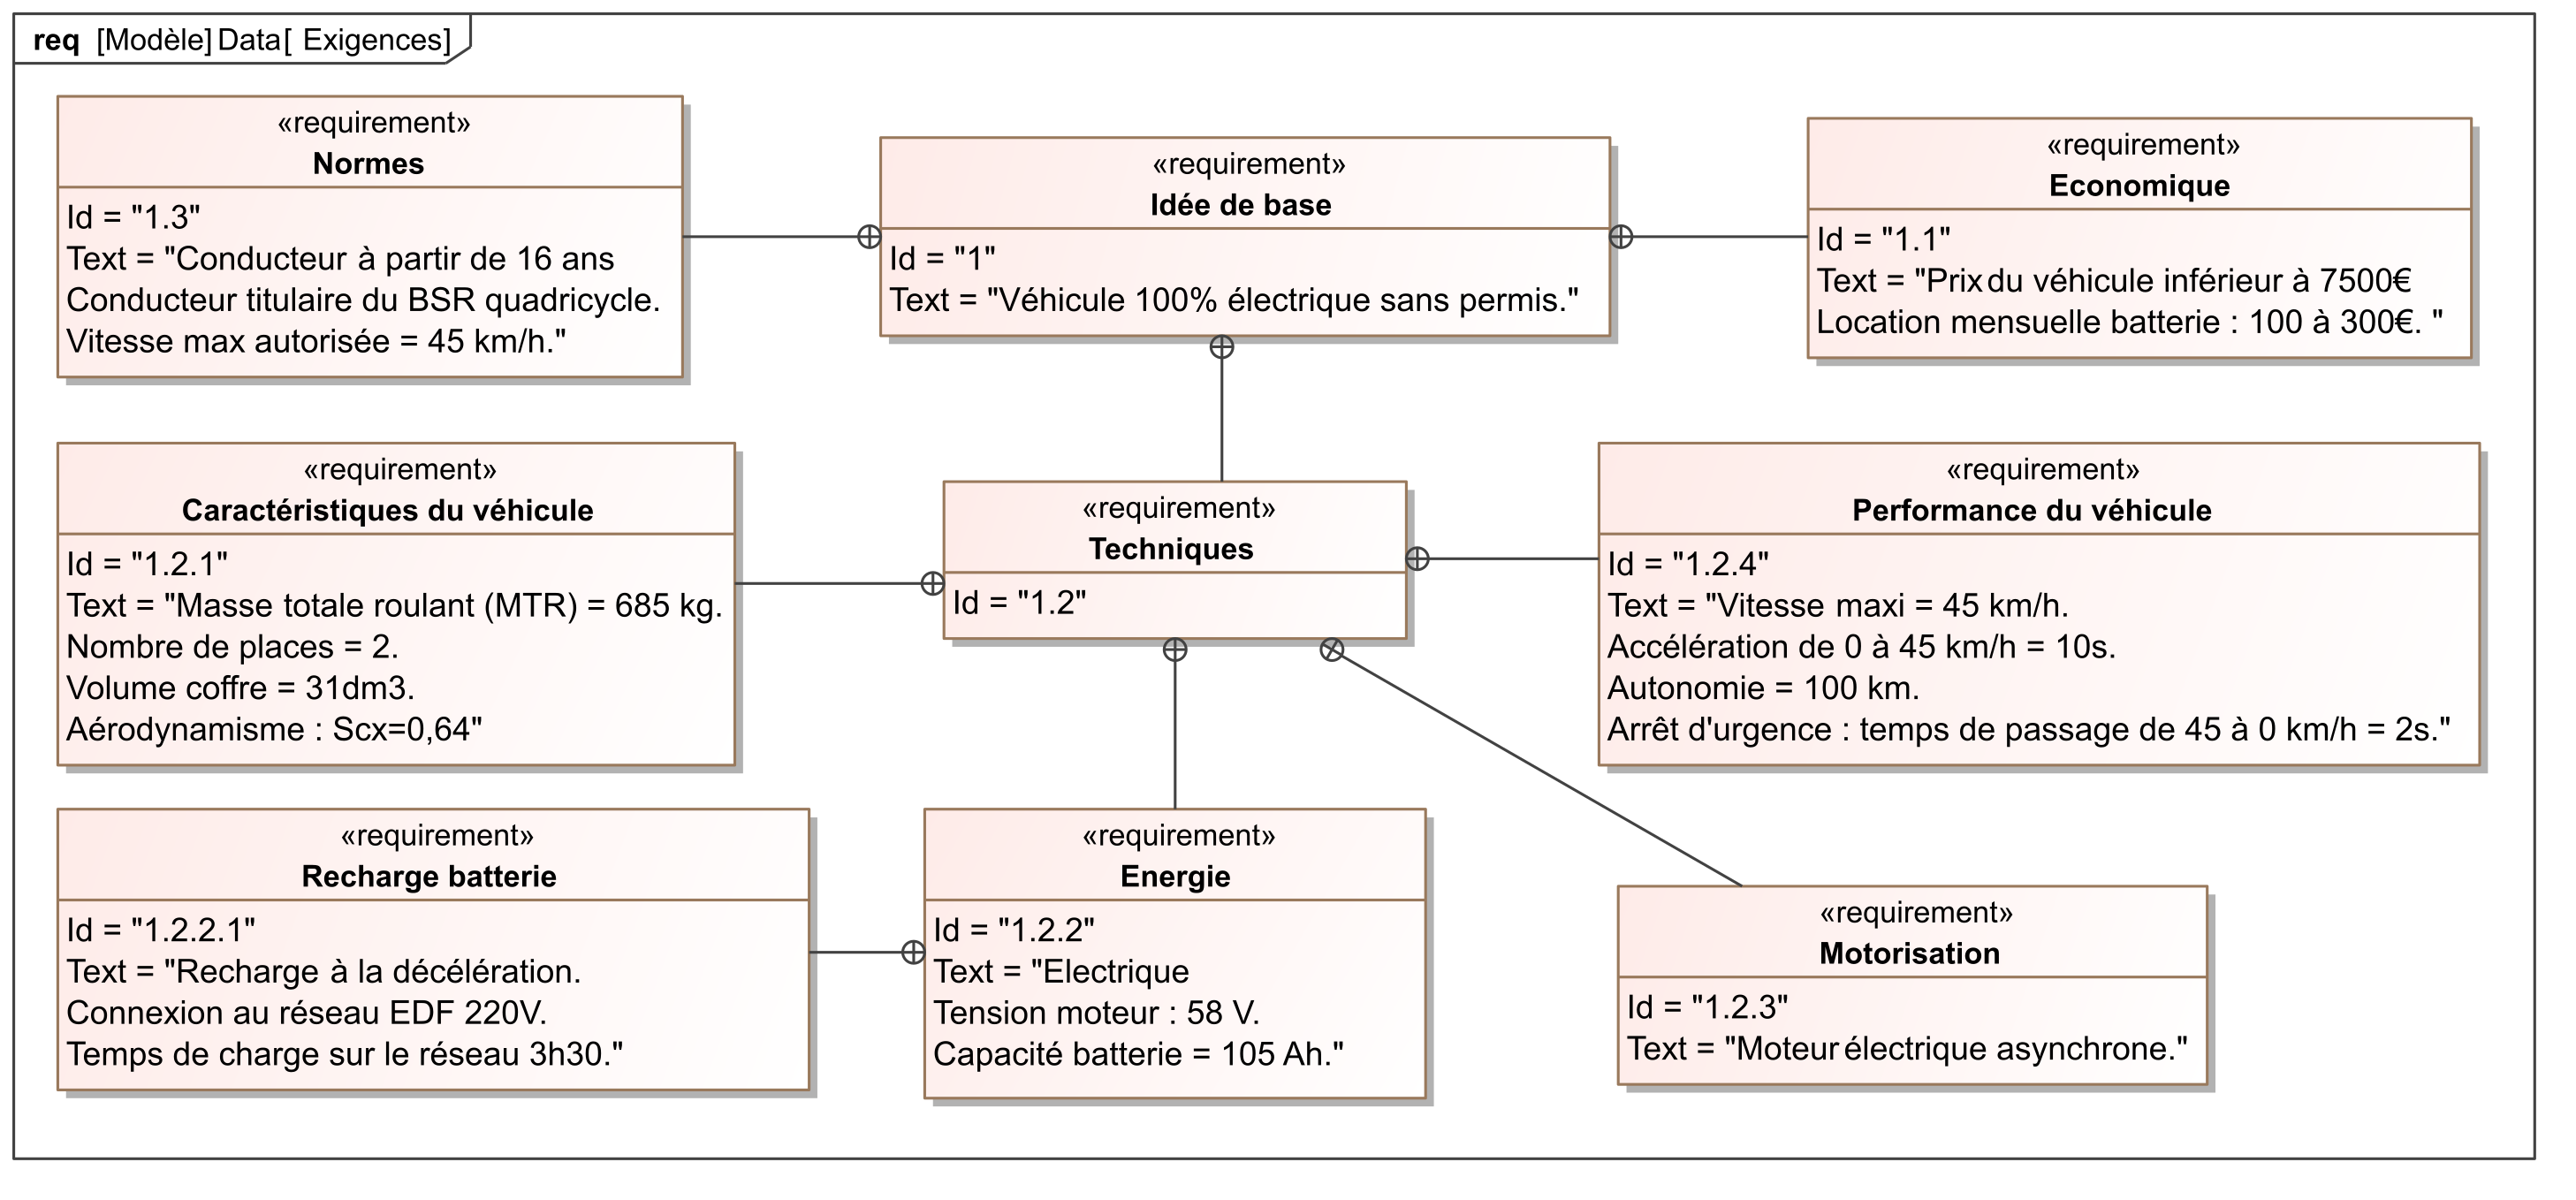
\includegraphics[width=\linewidth]{Exigences}
\end{center}

\subsection*{Choix du motoréducteur}


\begin{obj}
Mettre en place un modèle permettant de choisir un ensemble moto-réducteur afin d’obtenir les
exigences d’accélération et de vitesse.
\end{obj}

On donne le paramétrage et les données nécessaires pour cette modélisation.


\begin{center}
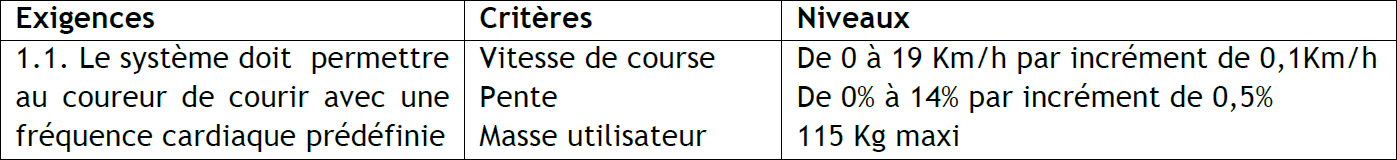
\includegraphics[width=\linewidth]{fig_02}
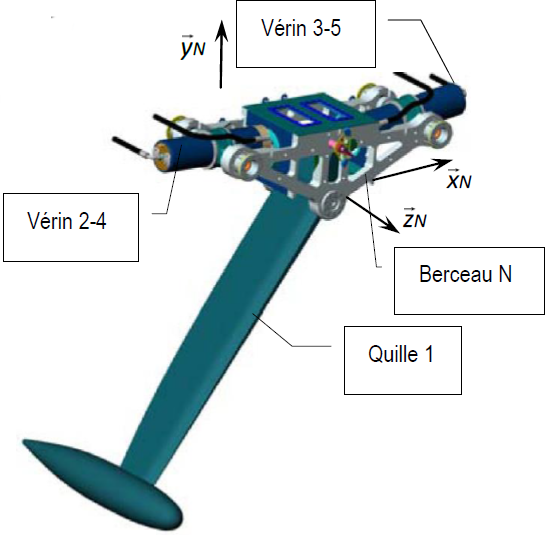
\includegraphics[width=\linewidth]{fig_03}
\end{center}


\textbf{Hypothèses générales : }
\begin{itemize}
\item le vecteur $\vect{z_0}$ est vertical ascendant et on notera $g$ l'accélération de la pesanteur;
\item le repère $\repere{O}{x_0}{y_0}{z_0}$ est galiléen;
Le centre de gravité de l’ensemble voiture et charges est supposé rester dans le
plan de symétrie de la voiture $\left(O,\vect{z_s},\vect{x_s}\right)$;
\item toutes les liaisons sont supposées parfaites à l’exception du contact roue -- sol;
\item les roues roulent sans glisser sur le sol en $I_i$;
\item le coefficient de résistance au roulement $\mu$ est identique pour tous les contacts
roue -- sol : $\mu = \si{3e-3}{m}$. On pose $\vect{I_1J_1}=\mu \vect{x_s}$, avec $\mu >0$
si le déplacement du véhicule est suivant $+\vect{x_s}$;
\item les frottements de l’air sur le véhicule seront négligés;
seules les roues arrière sont motrices.
\end{itemize}

\textbf{Actions mécaniques}
Le torseur des actions mécaniques du sol sur un ensemble, avant ou arrière, de roues
est :
$\torseurstat{F}{s}{i}=\torseurl{T_i\vect{x_s}+N_i\vect{z_s}}{\vect{0}}{J_i}$ avec $J_i \in \left(O,\vect{x_s},\vect{y_s}\right)$ et $i=1$ (roues arrières) ou 2 (roues avants). Le moteur permet d'appliquer un couple en 3 et 4 tel que 
$\torseurstat{F}{3}{4}=\torseurl{\vect{0}}{C_m\vect{y_0}}{-}$. 

\textbf{Masses et inerties : }
\begin{itemize}
\item le moment d'inertie du rotor moteur autour de son axe $\axe{A}{y_0}$ : $J_m =\SI{6e-3}{kg.m^2}$;
\item le moment d'inertie d'une roue autour de son axe $\axe{O_i}{y_0}$ : $J_R =\SI{0,1}{kg.m^2}$;
\item la masse du véhicule en charge : $m=\SI{685}{kg}$;
\item le centre de gravité du véhicule en charge sera noté $G$;
\item les autres inerties seront négligées.
\end{itemize}

\textbf{Grandeurs cinématiques :}
Soit $\omega_m$ la vitesse de rotation de l’arbre moteur 4 par rapport à 3, $\omega_{13}$ la vitesse de rotation des roues arrière 1 par rapport à 3 et $\omega_{23}$ la vitesse de rotation des roues avant 2 par rapport à 3.

On notera $r$ le rapport de transmission du réducteur tel que $\omega_m = r \omega_{13}$. On appellera $\vectv{G}{3}{0}=\vect{V}_{3/0}=v\vect{x_s}$la vitesse du véhicule.
Les roues ont un rayon $R = \SI{280}{mm}$.


\subsubsection*{Choix de l’ensemble moto-réducteur}
\subsubsection*{Équation de mouvement du véhicule}


\begin{obj}
Objectif : Déterminer l’équation de mouvement nécessaire pour choisir l’ensemble moto-réducteur.
\end{obj}

\textbf{Notations :}
\begin{itemize}
\item puissance extérieure des actions mécaniques du solide $i$ sur le solide $j$ dans le mouvement de $i$ par rapport à 0 : $\mathcal{P}\left( i \to j / 0\right)$;
\item puissance intérieure des actions mécaniques entre le solide $i$ et le solide $j$: $\mathcal{P}\left( i \leftrightarrow j\right)$ ;
\item énergie cinétique du solide $i$ dans son mouvement par rapport à 0 : $\mathcal{E}_c\left(i/0\right)$.
\end{itemize}

\subparagraph{}\textit{
\begin{itemize}
\item Écrire la forme générale du théorème de l’énergie puissance appliqué au véhicule en identifiant les différentes puissances extérieures, les différentes puissances intérieures et les énergies cinétiques des différents éléments mobiles en respectant les notations précédentes ;
\item déterminer explicitement les différentes puissances extérieures ;
\item déterminer explicitement les différentes puissances intérieures ;
\item déterminer explicitement les énergies cinétiques ;
\item en déduire une équation faisant intervenir $C_m$, $N_1$, $N_2$, $v$, $\omega_m$, $\omega_{1/0}$, $\omega_{2/0}$ …… ;
\item expliquer pourquoi l’équation obtenue n’est pas l’équation de mouvement du véhicule.
\end{itemize}
}
\ifprof
\begin{corrige}~\\
On isole l'ensemble du véhicule, et on a : 
\begin{itemize}
\item $\ec{E}{0} = \ec{1}{0}+\ec{2}{0}+\ec{3}{0}+\ec{4}{0}$;
\item $\pext{\overline{E}}{E}{0} = \pext{0}{1}{0}+\pext{0}{2}{0}+\pext{\text{pes}}{3}{0}$;
\item $\mathcal{P}_{\text{int, Liaisons}}=\pint{1}{3}{}+\pint{3}{2}{}+\pint{2}{4}{}$ car les liaisons à l'intérieur de l'isolement sont parfaites;
\item $\mathcal{P}_{\text{moteur}}=\pint{3}{4}{}= \torseurstat{F}{3}{4} \otimes \torseurcin{V}{4}{3}= C_m \omega_{4/3}$;
\item au final : 
$\dfrac{\dd \ec{1}{0}}{\dd t}+\dfrac{\dd \ec{2}{0}}{\dd t}+\dfrac{\dd \ec{3}{0}}{\dd t}+\dfrac{\dd \ec{4}{0}}{\dd t} =
\pext{0}{1}{0}+\pext{0}{2}{0}+\pext{\text{pes}}{3}{0}+C_m \omega_{4/3} $
\end{itemize}
Calcul des puissances extérieures :
\begin{itemize}
\item $ \pext{0}{1}{0} = \torseurstat{F}{0}{1} \otimes \torseurcin{V}{1}{0} $ 
$=\torseurl{T_1\vect{x_s}+N_1\vect{z_s}}{\vect{0}}{J_1} \otimes  \torseurl{\omega_{1/0} \vect{y_0}}{\vectv{I_1}{1}{0}+\vect{J_1I_1}\wedge \omega_{1/0} \vect{y_0}}{J_1}$ 

$=\torseurl{T_1\vect{x_s}+N_1\vect{z_s}}{\vect{0}}{J_1} \otimes  \torseurl{\omega_{1/0} \vect{y_0}}{-\mu\vect{x_s}\wedge \omega_{1/0} \vect{y_s}}{J_1}$ 
$=\torseurl{T_1\vect{x_s}+N_1\vect{z_s}}{\vect{0}}{J_1} \otimes  \torseurl{\omega_{1/0} \vect{y_0}}{-\mu\omega_{1/0}\vect{z_s}}{J_1}$ 

$= -\mu\omega_{1/0} N_1$.

\item $ \pext{0}{2}{0} = \torseurstat{F}{0}{2} \otimes \torseurcin{V}{2}{0}$ $= -\mu\omega_{2/0} N_2$.

\item $ \pext{\text{pes}}{3}{0} = \torseurstat{F}{\text{pes}}{3} \otimes \torseurcin{V}{3}{0} =\torseurl{-mg\vect{z_0}}{\vect{0}}{G} \otimes  \torseurl{\vect{0}}{v\vect{x_s}}{G} =-mvg\sin\alpha$.

\end{itemize}


Calcul des énergies cinétiques : 
\begin{itemize}
\item $\ec{1}{0} = \dfrac{1}{2} \cdot 2 J_r \omega_{1/0}^2  = J_r \omega_{1/0}^2$ (masse des roues négligée);
\item $\ec{2}{0} = J_r \omega_{1/0}^2$;
\item $\ec{3}{0} = \dfrac{1}{2}mv^2$;
\item $\ec{4}{0} = \dfrac{1}{2} J_m \omega_m^2$ (masse du rotor négligée).
\end{itemize}


En appliquant le théorème de l'énergie cinétique, on a :
$$
4 J_r \omega_{1/0} \dot{\omega}_{1/0} + m v \dot{v} + J_m \omega_m \dot{\omega}_m =  -\mu\omega_{1/0} N_1-\mu\omega_{2/0} N_2 -mvg\sin\alpha +C_m \omega_{4/3}. $$

Cette équation dépend des efforts dans les roues. Ce n'est donc pas une équation de mouvement.


\end{corrige}

\else
\fi


\subparagraph{}\textit{À partir des théorèmes généraux de la dynamique, déterminer une équation supplémentaire qui permet simplement de déterminer $(N_1 + N_2)$. Puis avec l’équation précédente, écrire l’équation de mouvement du véhicule.}
\ifprof
\begin{corrige}~\\
Pour exprimer $(N_1 + N_2)$ on peut isoler $E$ et appliquer le théorème de la résultante dynamique en projection sur $\vect{z_s}$. On a : 
$$
N_1 + N_2 + \left(-mg\vect{z_0}\right)\cdot \vect{z_s} = \vectg{G}{E}{0} \cdot \vect{z_s} \Rightarrow 
N_1 + N_2 -mg\cos \alpha = 0
$$

Et donc : 

$$4 J_r \omega_{1/0} \dot{\omega}_{1/0} + m v \dot{v} + J_m \omega_m \dot{\omega}_m =  -\mu\omega_{1/0} mg\cos \alpha -mvg\sin\alpha +C_m \omega_{4/3}. $$

\end{corrige}
\else
\fi

\subparagraph{}\textit{Déterminer en énonçant les hypothèses nécessaires les relations entre $(v, \omega_{10})$, $(v, \omega_{20})$ et $(\omega_{m}, \omega_{10})$. Montrer que l’équation de mouvement du véhicule peut se mettre sous la forme $\dfrac{rC_m(t)}{R}-F_r(t)=M_{eq}\dfrac{\text{d} v(t)}{\text{d} t}$ avec $F_r(t)$ fonction de $m$, $\mu$, $g$, $R$ et $\alpha$ et $M_{eq}$ fonction $m$, $J_m$, $J_R$, $R$ et $r$.}
\ifprof
\begin{corrige}~\\
En faisant l'hypothèse de roulement sans glissement en $I_1$ et $I_2$ on montre que $v = R\omega_{1/0}= R\omega_{2/0}$. De plus, $r\omega_{1/0}=\omega_m$ (défini ainsi dans le sujet).


On a donc : 
$$4 J_r \dfrac{v}{R}  \dfrac{\dot{v}}{R}  + m v \dot{v} + J_m \dfrac{rv}{R} \dfrac{\dot{v}r}{R} =  -\mu\dfrac{v}{R}  mg\cos \alpha -mvg\sin\alpha +C_m \dfrac{rv}{R} $$


$$  \Leftrightarrow \dot{v}\left(\dfrac{4 J_r }{R^2}   + m  +  \dfrac{J_mr^2}{R^2}  \right)=  -\mu\dfrac{1}{R}  mg\cos \alpha -mg\sin\alpha +C_m \dfrac{r}{R}. $$

En conséquences, $M=\dfrac{4 J_r }{R^2}   + m  +  \dfrac{J_mr^2}{R^2}$ et $F_r(t)=mg\left(\mu\dfrac{1}{R}  \cos \alpha +\sin\alpha\right)$

\end{corrige}
\else
\fi

\subsubsection*{Détermination du coefficient de résistance au roulement $\mu$}
\begin{obj}
Déterminer le coefficient de résistance au roulement $\mu$ suite à une expérimentation.
\end{obj}


\subparagraph{}\textit{En utilisant les résultats de l’essai routier effectué ci-dessous, il est possible de déterminer le coefficient de
résistance au roulement $\mu$. Proposer un protocole expérimental pour l’évaluer :
\begin{itemize}
\item justifier dans quelle phase se placer;
\item définir la variable mesurée;
\item définir les hypothèses nécessaires;
\item énoncer les équations utilisées pour déterminer $\mu$.
\end{itemize}}
\ifprof
\begin{corrige}~\\
En se plaçant à vitesse constante, on a $\dfrac{rC_m(t)}{R}-F_r(t)=0$.
Si le sol est horizontal, on a  $\alpha=0$ et $F_r(t)=mg\dfrac{\mu}{R}$ .

Ainsi, $\dfrac{rC_m(t)}{R}-mg\dfrac{\mu}{R}=0$ $ \Leftrightarrow \mu = \dfrac{rC_m(t)}{mg}$.

En réalisant l'applicaiton numérique lorsque la vitesse est constante, on a $m=\SI{685}{kg}$, $g=\SI{9,81}{m.s^{-2}}$, $C_m(t)=\SI{5}{Nm}$.
\end{corrige}
\else
\fi

\begin{center}
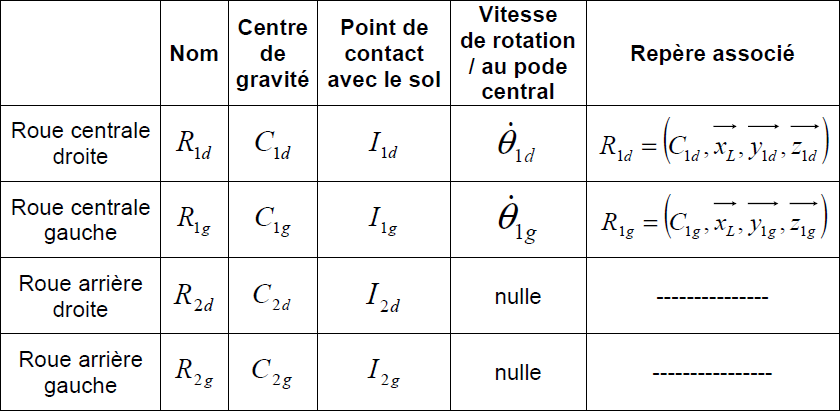
\includegraphics[width=\linewidth]{fig_04}
\end{center}


\subsubsection*{Choix du moto-réducteur}
\begin{obj}
Choisir un ensemble moto-réducteur afin d’obtenir les exigences d’accélération et de vitesse.
\end{obj}

Les courbes de l’évolution de l’accélération maximale $\dfrac{\text{d} v(t)}{\text{d} t}$
du véhicule obtenue pour 3 moteurs présélectionnés en fonction du rapport de transmission $r$ issues de l’équation de mouvement du véhicule précédente sont fournies sur le document réponse.




\subparagraph{}\textit{Déterminer la valeur minimale du rapport de transmission $r_{\text{mini}}$ pour les 3 moteurs proposés qui permet d’obtenir l’accélération maximale moyenne souhaitée dans le diagramme des exigences.}
\ifprof
\begin{corrige}~\\
\end{corrige}
\else
\fi


\subparagraph{}\textit{Déterminer la valeur maximale du rapport de transmission $r_{\text{max}}$ qui permet d’obtenir au moins la vitesse maximale du véhicule souhaitée dans le diagramme des exigences.}
\ifprof
\begin{corrige}~\\
\end{corrige}
\else
\fi


\subparagraph{}\textit{À partir des résultats précédents, choisir parmi les 3 moteurs proposés, celui qui respecte les exigences d’accélération et de vitesse souhaitées permettant la plus grande plage possible pour le rapport de transmission.}
\ifprof
\begin{corrige}~\\
\end{corrige}
\else
\fi


\subsubsection*{Validation du choix constructeur du moto-réducteur}
\begin{obj}
Valider le choix du moto-réducteur fait par le constructeur.
\end{obj}

\subparagraph{}\textit{À partir de la vue 3D du réducteur choisi par le constructeur, compléter le schéma cinématique du document réponse, calculer son rapport de transmission $r = \dfrac{\omega_{4/3}}{\omega_{4/3}}$ et conclure.}
\ifprof
\begin{corrige}~\\
\end{corrige}
\else
\fi


\begin{center}
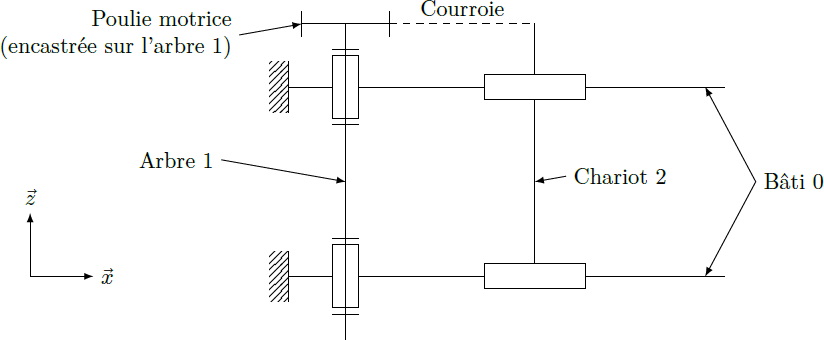
\includegraphics[width=\linewidth]{fig_05}
%\textit{}
\end{center}



\ifprof
%\end{multicols}
\else
\end{multicols}
\fi


